\documentclass[12pt]{letter}
\usepackage{german,a4,inputenc}
\usepackage{pdfpages}
% You need to adapt the information below and
% - insert your own reviewer suggestions
% - insert your own publications and talks
% - enter the number for the bibliographical information by hand
%    or follow the instructions (in BiblioInfo.tex) on how to generate them automatically


%\newcommand{\year}{2009}
% in case there is an error like "the \year already defined" please use the following command:
\renewcommand{\year}{2022}


\newcommand{\mefirst}{Cyrille Merleau}
\newcommand{\melast}{Nono Saha}
\newcommand{\me}{Nono Saha Cyrille Merleau}
\newcommand{\mystreet}{Kohlenstr. 16}
\newcommand{\mycity}{0407 Leipzig}
\newcommand{\mytel}{015257082636}
\newcommand{\myemail}{nonosaha@mis.mpg.de}
\newcommand{\mysupervisor}{Herrn \ Dr.\ Matteo Smerlak}
\newcommand{\thedean}{Martin Middendorf} % if female, change salutation!
\newcommand{\facultystreet}{PF 10 09 20}
\newcommand{\facultycity}{04009 Leipzig}
% defines the relative path for the autogenerated numbers in BiblioInfo.tex
\newcommand{\mypaths}{../} 
% Thesis title in English and German
\newcommand{\mytitle}{From RNA folding to inverse folding: a computational study}
\newcommand{\mytitleDE}{Von der RNA-Faltung zur inversen Faltung: eine computergestützte Studie}
\newcommand{\department}{Informatik} % or "Informatik" at your choice. 

\begin{document} \pagestyle{empty}
%\begin{flushleft}
\me        \hfill Leipzig, den 25. August 2022\\ 
\mystreet\\ 
\mycity \\
Tel.: \mytel \\
Email: \myemail

\end{flushleft}
\vspace*{0.2cm}
\begin{flushleft}
An den\\
Dekan der Fakult\"at f\"ur\\ 
Mathematik und Informatik\\
Universit\"at Leipzig\\
\facultystreet\\ 
\facultycity
\end{flushleft}

{\bf Betreff: Durchf\"uhrung meines Promotionsverfahrens}\\

Sehr geehrter Herr Prof.\ Dr.\ \thedean,

hiermit m\"ochte ich die Durchf\"uhrung meines Promotionsverfahrens im Fachgebiet \department zur Erlangung des Doktorgrades Doctor rerum naturalium (Dr.\ rer.\ nat.) an der Fakult\"at f\"ur Mathematik und Informatik der Universit\"at Leipzig beantragen. \\[.2cm]
Die Anfertigung der Dissertation wurde von \mysupervisor\ betreut. \\
Prof. Dr. Peter Stadler vom Institut für Informatik der Universität Leipzig befürwortet die Einreichung meiner Dissertation.\\
Mit freundlichen Gr\"u\ss en,
\vspace{2cm}

\me \\
 
{\bf Anlagen:} Dissertation (3 gebundene Exemplare), Zusammenfassung
der Dissertation (30 Exemplare), beglaubigte Kopie meiner Diplomurkunde,
tabellarischer Lebenslauf, Erkl\"arungen nach \textsection 6 1.5 der
Promotionsordnung, Verzeichnis der wissenschaftlichen Ver\"offentlichungen und Vortr\"age, Gutachtervorschl\"age.


%%% Local Variables: 
%%% mode: latex
%%% TeX-master: "dissdocuments"
%%% End: 

%\newpage
\begin{center}{\Large \bf Erkl\"arungen }\end{center}

\begin{itemize}
\item Ich erkenne die Promotionsordnung der Fakult\"at f\"ur Mathematik und Informatik der Universit\"at Leipzig vom 2. Mai 2013 in der Fassung der Ersten \"Anderungssatzung vom 16. Oktober 2017 an. \vspace{0.2cm}

\item Die eingereichte Arbeit wurde nicht in gleicher oder \"ahnlicher Form einer anderen Pr\"ufungsbeh\"orde zum Zwecke einer Promotion oder eines anderen Pr\"ufungsverfahrens vorgelegt. \vspace{0.2cm}

\item Es haben keine fr\"uheren erfolglosen Promotionsversuche stattgefunden. 
\vspace{0.2cm}

\end{itemize}

\vspace*{1.5cm}
\begin{flushleft}
...............................................\\
(\me)
\end{flushleft}

%%% Local Variables: 
%%% mode: latex
%%% TeX-master: "dissdocuments"
%%% End: 

%%%%%%%%%%%%%%%%%%%%%%%%%%%%%%%%%%%%%%%%%%%%%%%%%%%
%% Bibliographical Information 
%%%%%%%%%%%%%%%%%%%%%%%%%%%%%%%%%%%%%%%%%%%%%%%%%%
\begin{flushleft}{\bf Bibliographische Daten} \\\rule{120mm}{0.5mm}\end{flushleft}
\mytitle \\
(\mytitleDE)\\
\melast, \mefirst\\
Universit\"at Leipzig, Dissertation, \year \\
% NOTE: the number below are placed into files, which is useful, if
% you decide to generate them automatically (as detailed below). If
% you are the manual type, you can also just count them and insert a number.
%\input{\mypaths pages.num}Seiten, \input{\mypaths figs.num}Abbildungen, \input{\mypaths refs.num}Referenzen\\

% Automatizing the counters:
% General: since you need the counters here, but the information is
% only present in your thesis file, one needs to write them to disk
% (the *.num files above)  during typesetting the thesis. 
% You can do so, by using the newfile latex package (just google it)
% and insert the following lines in you main file:
%
% \newoutputstream{pages}
% \openoutputfile{pages.num}{pages} 
% \addtostream{pages}{\arabic{page}}
% \closeoutputstream{pages}
% 
% They need to be adapted for each of the following counters:
%
% Page counter:
% The page counter is already defined in latex: as you see above, its
% value is written do disk by issueing \arabic{page} in the newfile
% constructs.
%
% Figure counter: 
% If you have defined a figure environment, e.g. 
% \newcommand{\Figure}[3][htp]{
%  \addtocounter{AllFigures}{1}
%  \begin{figure}[#1]
%    \centering % if Figure Labels don't work remove this
%    \includegraphics[width=\textwidth]{Figures/FIG_#2.pdf}
%    \caption{#3}  
%    \label{#2}
%  \end{figure}}
%
% If you have not defined a figure environment, use query replace, e.g.
% end{figure} by addtocounter{AllFigures}{1} \\end{figure}
% If your thesis is spread out over multiple .tex files use reftex-query-replace-document
%
% then (as above), you can just insert the counter increment.
% Before this definition you need to define the counter:
% \newcounter{AllFigures}
% Then you need to adapt the writefile lines above to use the counter
% AllFigures and write to the file figs.num
%
% Ref counter:
% To automatically count the number of references, it seemed easiest
% to insert a counter into the .bbl file produced by BiBTeX. Since the
% .bbl-file is regenerated often, you need to insert the counter in
% the definition of your BiBTeX-style, i.e. the corresponding .bst
% file. Which one you use is shown in the BiBTeX output. Once you have
% found it, look for the place where the \bibitem is inserted, e.g.
% 
% FUNCTION {output.bibitem}
%{ newline$
%  "\addtocounter{Cites}{1} \bibitem[" write$
%  label write$
%  "]{" write$
%  cite$ write$
%  "}" write$
%  newline$
%  ""
%  before.all 'output.state :=
%}
%
% where the \addtocounter{Cites}{1} was newly inserted. And again the
% counter Cites needs to be defined somewhere in your TeX code:
% \newcounter{Cites}
%
% OK, once you have confirmed that these number are written to the
% hard drive and that the relative paths are correct, you should never
% have to worry about counting references, figures, or pages again. 


%%% Local Variables: 
%%% mode: latex
%%% TeX-master: "dissdocuments.tex"
%%% End: 
%%use in documents with \subfile{tex/title}
\documentclass[../master.tex]{subfiles}

\begin{document}
\begin{abstract}
    \thispagestyle{plain}
    \setcounter{page}{2}

	RNA molecules are ubiquitous in living organisms.
	Besides their role in translating genetic information into functional, often catalytically active proteins, various classes of RNA molecules are capable of catalysis themselves.
	Their capability to carry heritable information and perform certain functions makes them promising candidates for pre-cellular self-replicating systems exhibiting Darwinian evolution.
	One such molecule is the \textit{Azoarcus} group I intron, which has been shown to catalyze self-assembly from smaller fragments.
	Finding an abundance of similar RNA molecules could strengthen the significance of RNA emerging prior to proteins in the origin of life, a view known as the RNA world hypothesis.
	
	In this thesis, I employ computational methods based on thermodynamics in order to design RNA sequences that are structurally similar to the \textit{Azoarcus} group I intron, motivated by the close relation of RNA structure and function.
	
	In general, RNA structure is hierarchical, and efficient prediction of secondary structure from RNA sequence is possible, facilitating the reverse process of finding sequences given a secondary target structure.
	However, the structure of the \textit{Azoarcus} group I intron contains a \emph{pseudoknot} related to its function.
	This feature is usually considered to be part of the tertiary structure.
	Prediction of general \emph{pseudoknots} has been shown to be NP-complete, and algorithms restricted to certain classes of \emph{pseudoknots} are still more complex than pure secondary structure prediction methods.
	
	The herein described design process accounts for this feature without explicitly modelling it, allowing to apply efficient secondary structure algorithms during RNA design while only requiring structure prediction methods with \emph{pseudoknots} for verification post-design.
	
\end{abstract}
\end{document}


%\includepdf{Short_CV.pdf}
%%%%%%%%%%%%%%%%%%%%%%%%%%%%%%%%%%
%% Selbst\"andigkeitserkl\"arung
%%%%%%%%%%%%%%%%%%%%%%%%%%%%%%%%%
\newpage
\begin{center}
{\bf Selbstst\"andigkeitserkl\"arung}
\end{center}
Hiermit erkl\"are ich, die vorliegende Dissertation selbst\"andig und ohne
unzul\"assige fremde Hilfe angefertigt zu haben. Ich habe keine anderen
als die angef\"uhrten Quellen und Hilfsmittel benutzt und s\"amtliche 
Textstellen, die w\"ortlich oder sinngem\"a{\ss} aus ver\"offentlichten oder unver\"offentlichten Schriften entnommen wurden, und alle Angaben, die auf m\"undlichen Ausk\"unften beruhen, als solche kenntlich gemacht. 
Ebenfalls sind alle von anderen Personen bereitgestellten Materialien 
oder erbrachten Dienstleistungen als solche gekennzeichnet.\\
\\
\begin{flushleft}
Leipzig, den 25. August 2022
\end{flushleft}
\vspace*{0.5cm}
\begin{flushleft}
$\ldots\ldots\ldots\ldots\ldots\ldots\ldots\ldots\ldots$\\
{\small(\me)}
\end{flushleft}
\includepdf{Formloser_Antrag.pdf}
\newpage
\begin{center}
{\Large \bf 
Gutachtervorschl"age}\vspace{0.5cm}
\end{center}

Folgende Personen w\"aren aufgrund ihrer fachlichen Kompetenz als Gutachter f\"ur diese Dissertation besonders geeignet:
\begin{itemize}
\item Prof.\ Dr.\ J\"urgen Jost\\
  Max-Planck-Institut f"ur Mathematik in den Naturwissenschaften\\
  Inselstr.\ 22-26\\
  D-04103 Leipzig\\
  email: jjost@mis.mpg.de\\
  Tel: 0341 9959 552\\
  Fax: 0314 9959 555\\

\item Prof.\ Dr.\ Maneesh Sahani\\ 
 Gatsby Computational Neuroscience Unit\\
 Alexandra House - 17 Queen Square\\
 London, WC1N 3AR, United Kingdom\\
 email: maneesh@gatsby.ucl.ac.uk\\
 Tel: +44 20 7679 5360\\
 Fax: +44 20 7679 1173\\

\item Prof.\ Dr.\ Rudolf R\"ubsamen\\
 Institut f\"ur Biologie II\\
 Universit\"at Leipzig\\
 Talstra\ss e 33\\
 D-04103 Leipzig\\
 email: rueb@rz.uni-leipzig.de\\
 Tel: 0341 9736 740\\
 Fax: 0341 9736 848\\

\item Prof.\ Dr.\ Shihab Shamma\\
Neural Systems Laboratory\\
Institute for System Research\\
2202 A.\ V.\ Williams Building\\
University of Maryland\\
College Park, MD 20742, USA\\
email: sas@umd.edu\\
Tel: +1 301 405 6596\\
Fax: +1 301 314 9920\\
\end{itemize}

%%% Local Variables: 
%%% mode: latex
%%% TeX-master: "dissdocuments"
%%% End: 

\includepdf{Befürwortung_Nono_Saha_Cyrille_Merleau.pdf}
\includepdf[pages={1-},]{Full_CV.pdf}
\includepdf{MSC_CS.pdf}
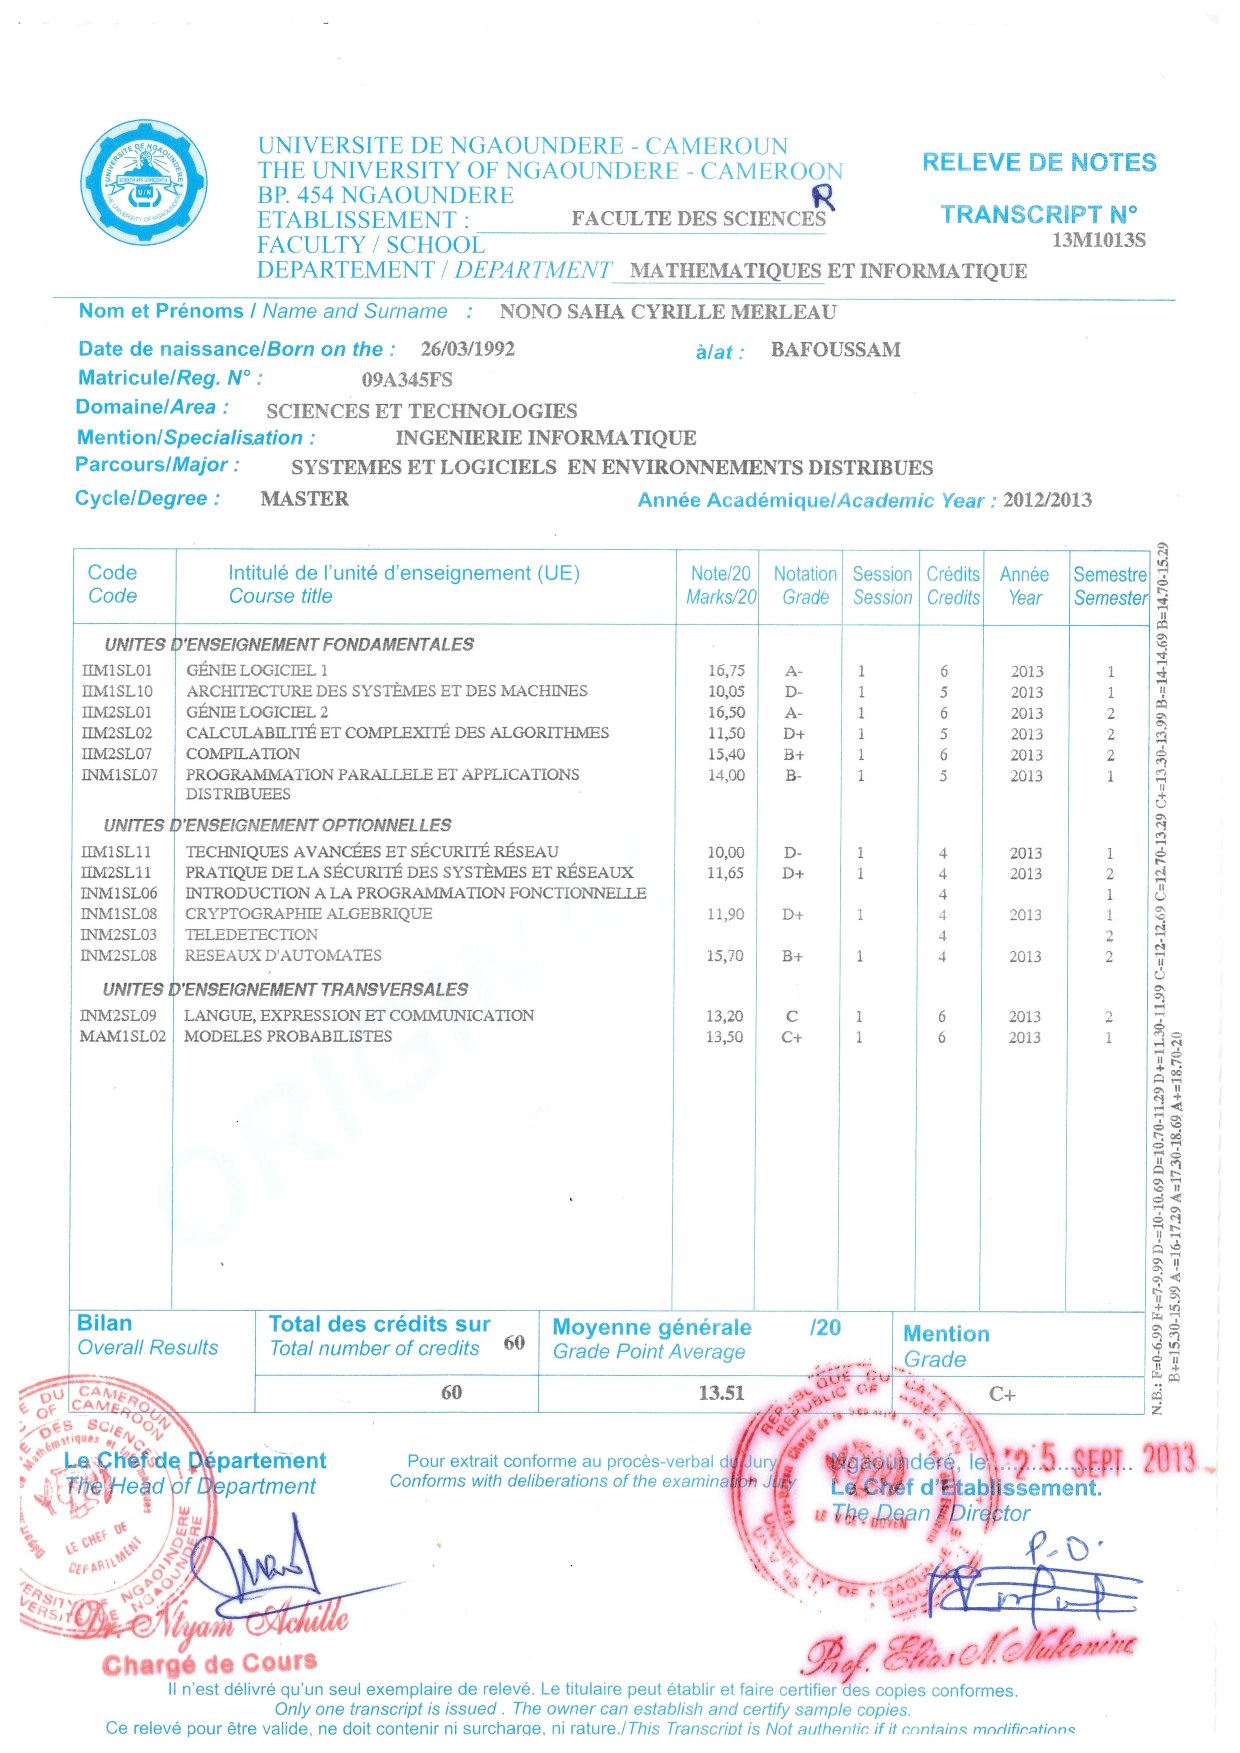
\includepdf{MSc_CS_transcript_Y1.pdf}
\includepdf{MSc_CS_transcript_Y2.pdf}
\includepdf{MSc_Maths_AIMS.pdf}
\includepdf{Msc_Maths_UL.pdf}
\includepdf{MSc-Transcript_Maths.pdf}
\includepdf{Bachelor_Certificate.pdf}
\end{document}
